\section{Data Flow Diagrams}
\subsection{Current System Context Diagram}
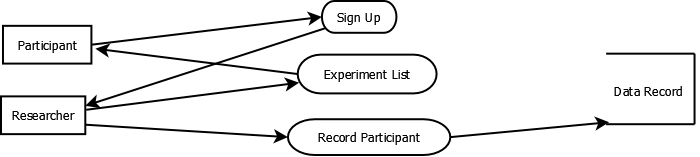
\includegraphics[width=6in]{../other/data-flow-diagrams/current_system_context_diagram.png}\\
The current system requires the researcher to post an experiment (Experiment List), with the Participant then seeing the experiment from the experiment list and signing up.  The researcher then gets the participants information and records the participant information into their current data record system.

\subsection{Current System Level 0 Data Flow Diagram}
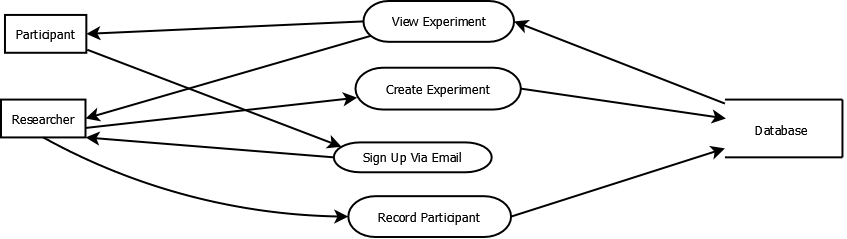
\includegraphics[width=6in]{../other/data-flow-diagrams/current_system_level0.png}\\
In the level zero data flow diagram, the flow remains the same, but the participant is signing up via email, while the researcher must explicitly create the experiment to be put on the data base (for this definition of data base the team is including a peg board of information or a campus email or similar types of information distribution).

\subsection{Proposed System Context Diagram}
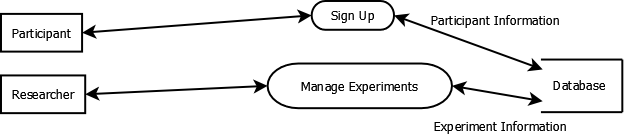
\includegraphics[width=6in]{../other/data-flow-diagrams/new_system_context.png}\\
In the proposed system, the researcher will manage experiments via an computer data base.  This same data base will let the user sign up and keep their information for the experiment.

\subsection{Proposed System Level 0 Data Flow Diagram}
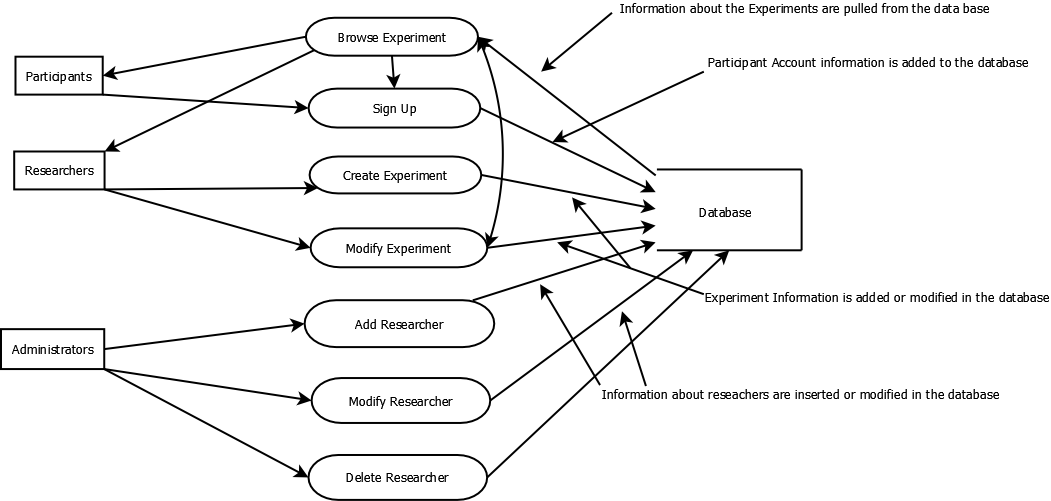
\includegraphics[width=6in]{../other/data-flow-diagrams/new_system_level_0.png}\\
Now, in the level 0 diagram, creating and experiment and modifiying an experiment are explicitly different, but both have data being stored on the computer data base.  The participant now browses the experiment and then signs up, instead of the two being combined.  The data entered by the participant will be saved on the data base.  Another actor, the administrator, will have the ability to add a researcher or modifiy a researcher.  All of the data about the researchers will be placed on the computer data base.

\subsection{Proposed System Level 1 Data Flow Diagram for Sign up}
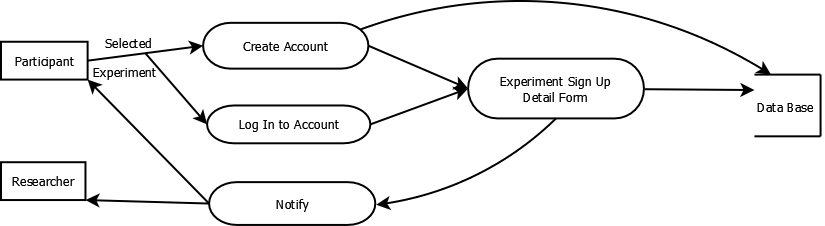
\includegraphics[width=6in]{../other/data-flow-diagrams/new_system_level_21.png}
When signing up the participant has selected a specific experiment to begin with.  Then, the participant creates an account, with the information being stored in the computer data base, or logs into their account.  Next the participant will select a time and confirm that they conform to the qualifications of the experiment.  This information will be stored in the computer data base.  After finishing sign up, the researcher and participant will be notified via email of the new participant.